\subsection{Grundlagen der Energiebilanzierung}

%%%%%%%%%%%%%%%%%%%%%%%%%%%%%%%%%%%%%%%%%%%%%%%%%%%%%%%%%%%%%%%%%%%%%%%%%%%%%%%%%%%%%%%%%%%%%%%%%%%%%%%%%%%%%%%%%%%%%%%%%%%%%%%%%%%%%%%%%%%%%%%%%%%%%%%%%%%%%%%%%%%
\subsubsection{Anwendungskontext der Energiebilanz}

Bilanzierung ist ein Konzept, welches in unterschiedlichen Einsatzbereichen Verwendung findet. 
Die DIN EN ISO 50001:2018-12 setzt den Schwerpunkt auf die fortlaufende Verbesserung der energiebezogenen Leistung (\cite[Kapitel 0.2]{DIN50001.2018}). 
Folglich hat vor allem die Energiebilanz im Energiemanagement nach der DIN EN ISO 50001:2018-12 eine große Relevanz und rückt in den Fokus 
dieser Forschungsarbeit.
Auch die Festlegung auf Organisationen des tertiären Wirtschaftssektors hat Auswirkungen auf die Betrachtungsweise der Bilanzierung. Denn in Organisationen 
mit immateriellen Dienstleistungen spielt die Gebäudeenergie eine vorrangige Rolle zur Verbesserung der energiebezogenen Leistung (\cite[S. 3]{Fichera.2020}).
Dies lässt sich beispielhaft an der Abbildung \eqref{fig:Energieverbrauch_Wärme_DE} darstellen.

\begin{figure}[H]
    \centering
    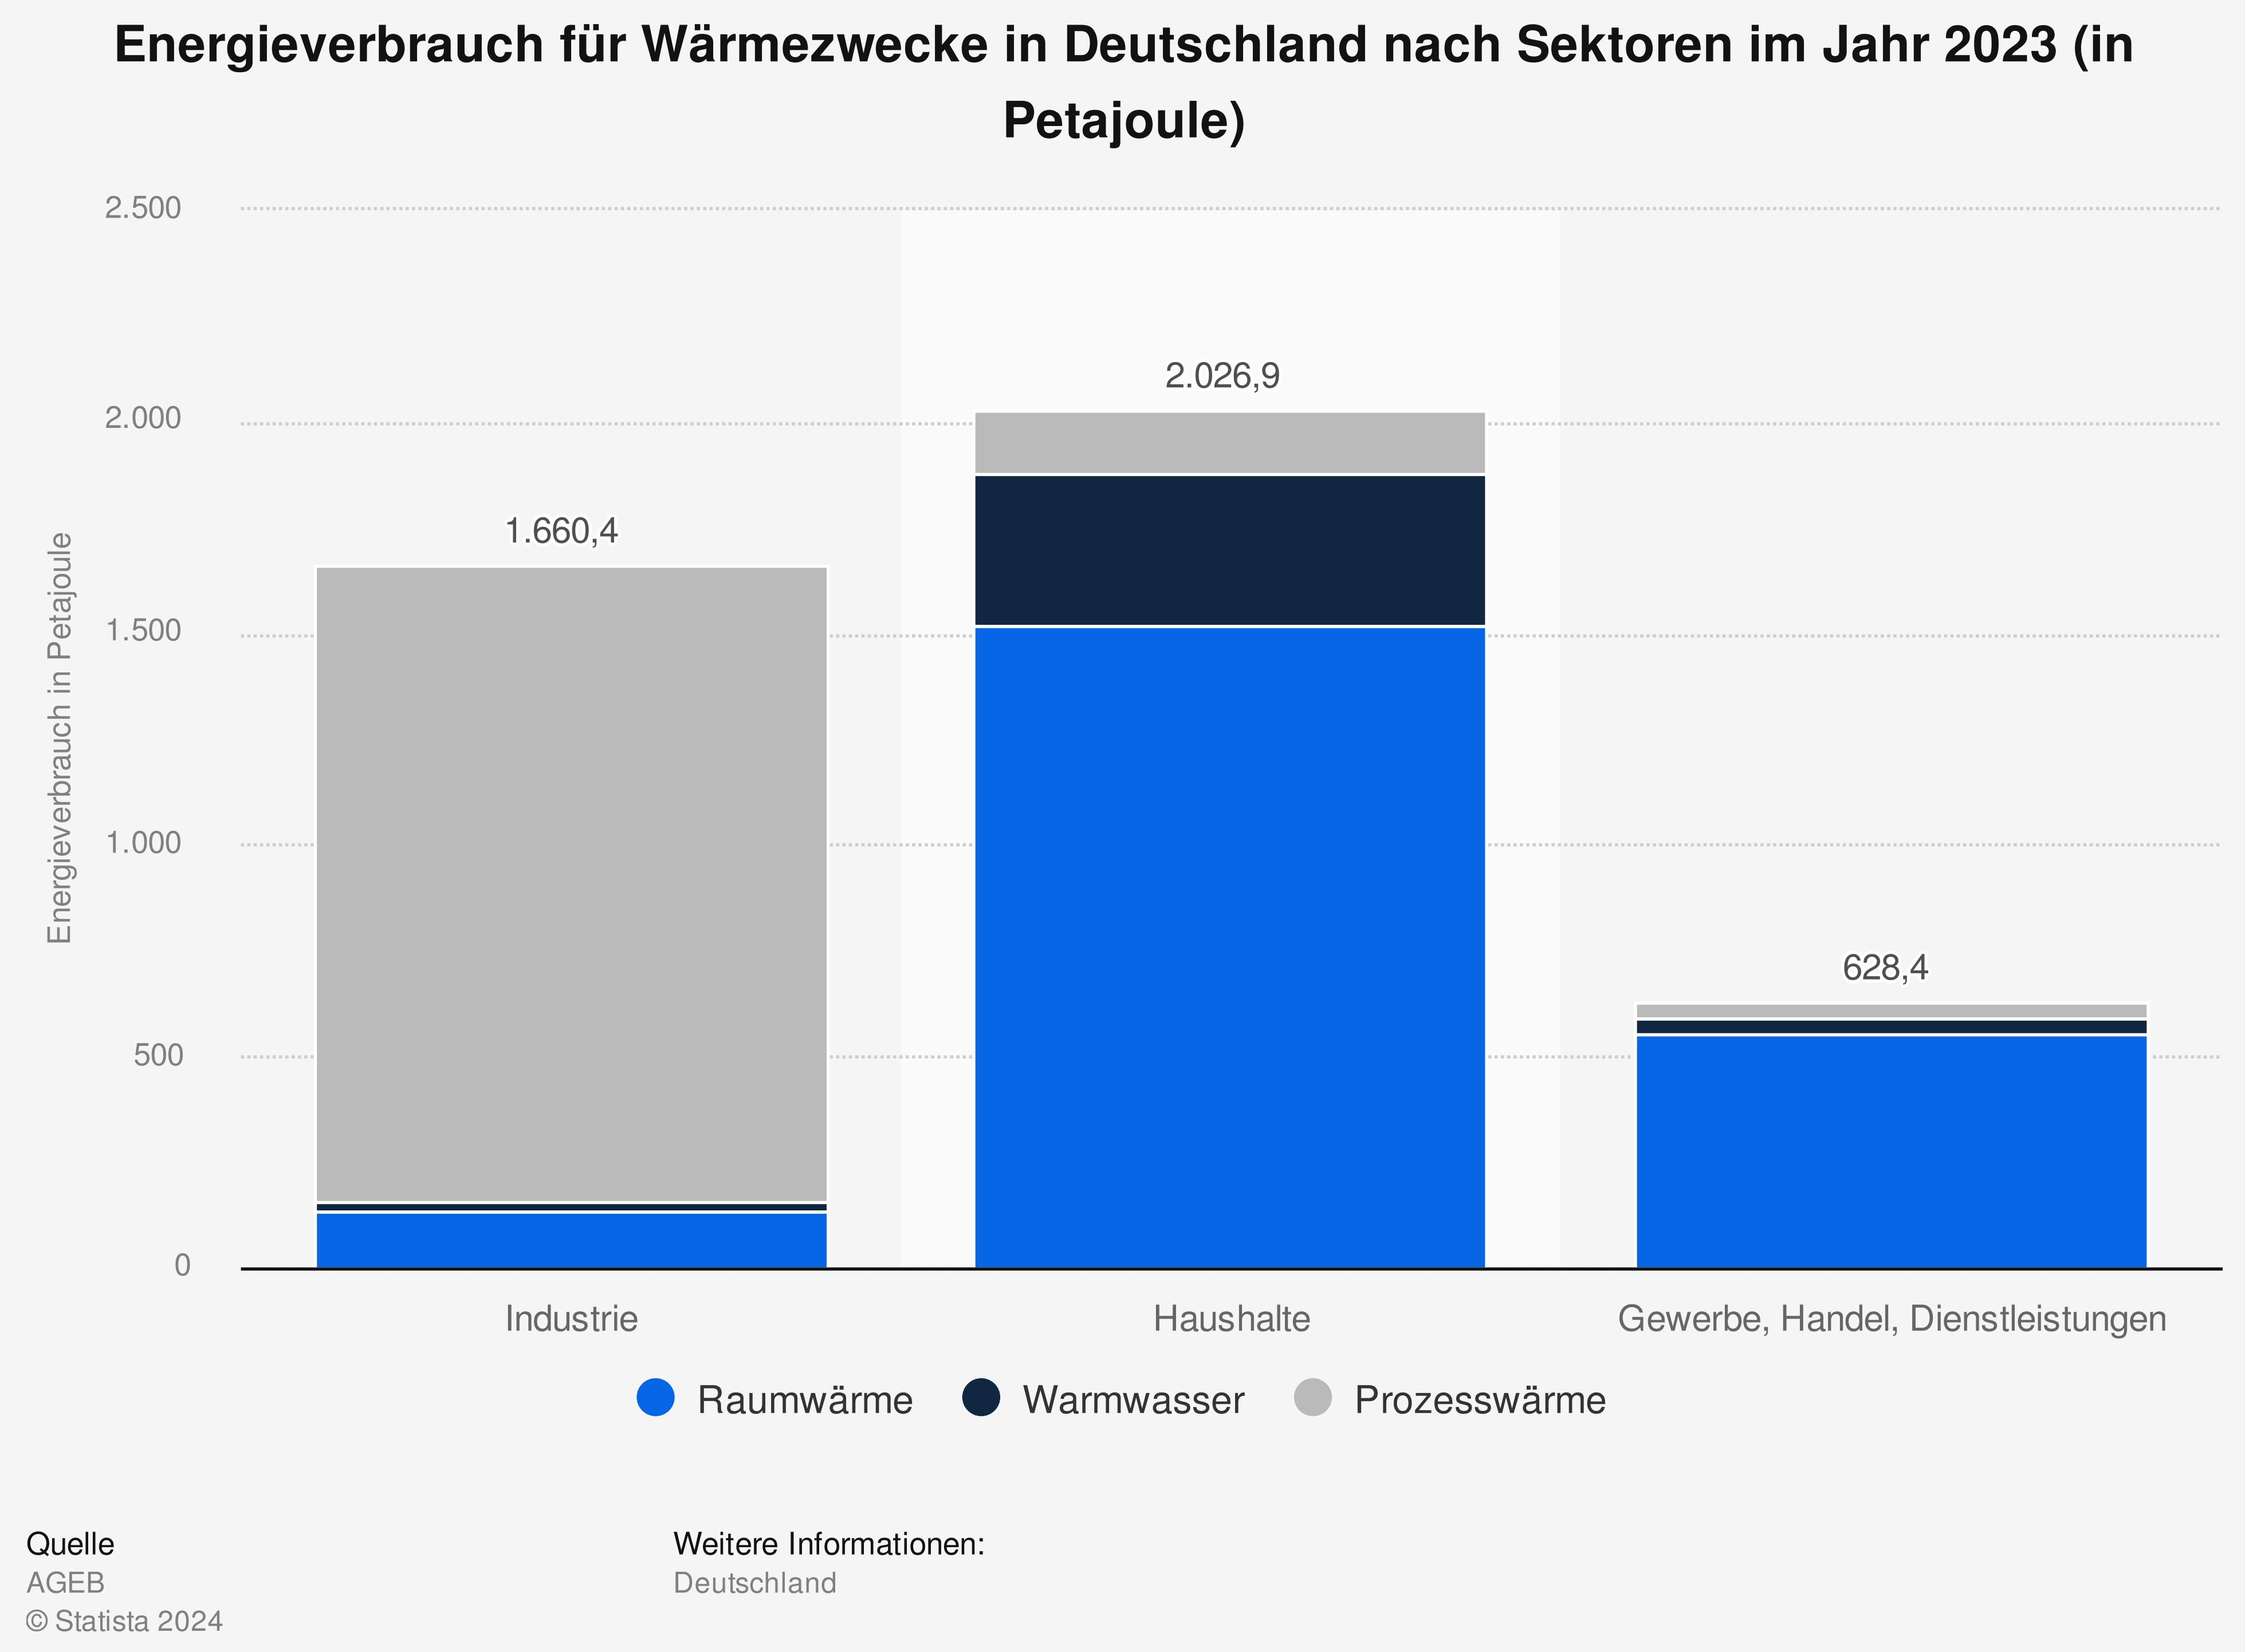
\includegraphics[width=0.85\textwidth]{../../Ressourcen/Abbildungen/Energieverbrauch_für_Wärmezweck_DE.jpg}
    \caption{Energieverbrauch für den Wärmezweck in Deutschland (Dargestellt von AGEB (2024))}
    \label{fig:Energieverbrauch_Wärme_DE}
\end{figure}

Die Abbildung \ref{fig:Energieverbrauch_Wärme_DE} zeigt den Energieverbrauch für Wärmezwecke in Deutschland im Jahr 2023, aufgeschlüsselt nach Sektoren. 
Während der industrielle Sektor einen hohen Anteil an prozessbezogener Wärme aufweist, 
spielt im Dienstleistungssektor die Raumwärme eine dominante Rolle.
Diese Statistik bekräftigt die Aussage von Fichera (2020, S. 3), dass bei der Verbesserung der energiebezogenen Leistung in Organisationen des tertiären 
Wirtschaftssektors energiebezogene Prozesse und Technologien im Gegensatz zur Gebäudeenergie eine untergeordnete Bedeutung haben.

Im Rahmen der Bestimmung des Gesamtenergiebedarfs eines Gebäudes über den Lebenszyklus wird vor allem der Gebäudebetrieb betrachtet (\cite[S. 133]{Musall.2015}).
Die sogenannte Graue Energie wird üblicherweise als kumulierter, nicht erneuerbarer Primärenergieaufwand beschrieben, der alle vor- und nachgelagerten Prozesse 
der verwendeten Baustoffe und Materialien sowie der technischen Anlagen umfasst (\cite[S. 133]{Musall.2015}). 
Die Arbeit grenzt sich von der Energiebilanzierung der grauen Energie ab und legt den Fokus auf den Gebäudebetrieb.
Im folgenden wird folglich die Energiebilanzierung im Rahmen des Gebäudebetriebs von Organisationen des tertiären Wirtschaftssektors 
betrachtet.

%%%%%%%%%%%%%%%%%%%%%%%%%%%%%%%%%%%%%%%%%%%%%%%%%%%%%%%%%%%%%%%%%%%%%%%%%%%%%%%%%%%%%%%%%%%%%%%%%%%%%%%%%%%%%%%%%%%%%%%%%%%%%%%%%%%%%%%%%%%%%%%%%%%%%%%%%%%%%%%%%%%

\subsubsection{Konzept}
Im beschriebenen Kontexts rückt die verfahrenstechnische Perspektive der Bilanzierung in den Fokus. 
In der Verfahrenstechnik wird eine Bilanz in drei Bilanzgleichungen unterteilt: die Massenbilanz, die Energiebilanz und die Impulsbilanz (\cite[S. 66]{Rönsch.2015}).
Wie im Kontext bereits erörtert liegt der Fokus im Problemraum dieser Arbeit auf der Energiebilanz.
Die Energiebilanz beruht auf dem Energieerhaltungssatz (\cite[S. 66]{Rönsch.2015}), der das Prinzip der Erhaltung der Energie ausdrückt 
(\cite[S. 57]{Baehr.1966}). 
Der Energieerhaltungssatz bezieht sich auf alle Erscheinungsformen, in denen Energie auftritt, und besagt, dass es 
unmöglich ist, Energie zu erzeugen oder zu vernichten (\cite[S. 57]{Baehr.1966}).
Für zu bilanzierende Systeme bedeutet dies, dass die Energie in einem abgeschlossenen, adiabaten System über die Zeit konstant ist 
(\cite[S. 66]{Rönsch.2015}). 
Adiabat bedeutet dass das System keine Wärme mit seiner Umgebung austauscht (\cite[S. 66]{Rönsch.2015}).
Für Systeme, die in der Lage sind, Energie zu speichern, impliziert diese Eigenschaft dass die darin gespeicherte Energie gleich der 
Differenz aus ein- und austretenden Energieströmen ist (\cite[S. 66f.]{Rönsch.2015}).
Für offene, nicht-adiabate Systeme ohne Speicherfähigkeit gilt, dass die Differenz der ein- und austretenden Energieströme null ist (\cite[S. 66f.]{Rönsch.2015}).
Das von Rönsch (2015, S. 66f.) beschriebene Verhalten eines Systems bezüglich der Energiespeicherung lässt sich mathematisch vereinfacht mit der Gleichung 
\eqref{energiebilanzierungsgleichung_Rönsch} darstellen:

\begin{equation}
E_{\text{gespeichert}} = \sum E_{\text{eingang}} - \sum E_{\text{ausgang}}
\label{energiebilanzierungsgleichung_Rönsch}
\end{equation}

\begin{description}
    \item \(E_{\text{gespeichert}}\): Im System gespeicherte Energie.
    \item \(E_{\text{eingang}}\): Energie eines eintretenden Energiestroms.
    \item \(E_{\text{ausgang}}\): Energie eines austretenden Energiestroms.
    \item Für offene, nicht-adiabate Systeme ohne Energiespeicher gilt:
    \[
    E_{\text{gespeichert}} = 0
    \]
    \item In diesem Fall ist die zugeführte Energie gleich der abgegebenen Energie (vgl. Gleichung \eqref{energiegleicheit_Rönsch}).
\end{description}

\begin{equation}
    \sum E_{\text{eingang}} = \sum E_{\text{ausgang}}
    \label{energiegleicheit_Rönsch}
\end{equation}

Rönsch (2016) kategorisiert somit zu bilanzierende System in speicherfähige und nicht speicherfähige Systeme.
Gleichung \eqref{energiegleicheit_Rönsch} beschreibt das Verhalten der ein- und austretenden Energieströme, welches für alle 
nicht speicherfähigen Systeme gelten muss.
Folglich stehen Energiespeicher im Zusammenfassung mit der Energiebilanz eines Systems und müssen bei der Bilanzierung berücksichtigt werden.
Energiespeicher können immer dann eingesetzt werden wenn Energie bereitsteht aber nicht unmittelbar genutzt wird (\cite[S. 1]{Rathgeber.2018}).
Der Speicher kann Energie aufnehmen und zu einem späteren Zeitpunkt oder an einem anderen Ort wieder abgeben (\cite[S. 1]{Rathgeber.2018}).
Energiespeicher werden nach Form der bereitgestellten Energien zwischen: Elektrizität, mechanische Energie, chemische Energie und Thermische 
Energie (\cite[S. 1]{Rathgeber.2018}).


Ein weiterer Ansatz zur Bilanzierung aus verfahrenstechnischer Perspektive wird durch die von Ahrendts (2014, Kapitel 1.5) aufgestellte Bilanzgleichung eines 
thermodynamischen Systems adressiert.
Der Gleichung liegt der Fakt zugrunde, dass sich für jede mengenartige Zustandsgröße, die über die Grenze eines Systems transportiert wird, eine Bilanz aufstellen lässt 
(\cite[Kapitel 1.5]{Ahrendts.2014}).
Die Bilanzgleichung (vgl. Gleichung \eqref{BilanzierungsgleichungAhrendt} und \eqref{BilanzierungsgleichungAhrendtStrom}) 
bildet die ein- und austretende Ströme sowie im System enthaltene Energiequellen und -senken auf die Geschwindigkeit der Änderung des Bestands der 
zu bilanzierenden Zustandsgröße im System ab (\cite[Kapitel 1.5]{Ahrendts.2014}).

\begin{equation}
    \frac{dX_{\text{j}}}{d\tau} = (\sum \dot{X}_{\text{j,e}} - \sum \dot{X}_{\text{j,a}}) + (\dot{X}_{\text{j,Quell}} - \dot{X}_{\text{j,Senk}})
    \label{BilanzierungsgleichungAhrendt}
\end{equation}

\begin{description}
    \item \(X_{\text{j}}\): Zustandsgröße.
    \item \(\tau\): Zeitintervall.
    \item \(X_{\text{j,e}}\): Über die Systemgrenze zufließende Zustandsgröße.
    \item \(X_{\text{j,a}}\): Über die Systemgrenze abfließende Zustandsgröße.
    \item \(X_{\text{j,Quell}}\): Quellen der Zustandsgröße im System.
    \item \(X_{\text{j,Senk}}\): Senken der Zustandsgröße im System.
\end{description}


\begin{equation}
    \dot{X}_{\text{j}} = \lim_{\Delta\tau \to 0} \Delta X_{\text{j}}/ \Delta\tau
    \label{BilanzierungsgleichungAhrendtStrom}
\end{equation}

\begin{description}
    \item \(X_{\text{j}}\): Zustandsgröße.
    \item \(\Delta X_{\text{j}}\): Menge der Größe \(X_{\text{j}}\) im Zeitintervall \(\Delta \tau\).
    \item \(\Delta \tau\): Zeitintervall.
\end{description}


 

Die Gleichung \eqref{BilanzierungsgleichungAhrendt} in Verbindung mit \eqref{BilanzierungsgleichungAhrendtStrom} beschreibt die Geschwindigkeit der Änderung des Bestands der Größe
\(X_{\text{j}}\) als Summe der Differenzen zwischen den über die Systemgrenze zu- und abfließenden Strömen der Zustandsgröße
\(X_{\text{j}}\) sowie den Quell- und Senkströmen der Zustandsgröße \(X_{\text{j}}\) innerhalb des Systems.  
Zur zweckmäßigen Anwendung der Gleichung \eqref{BilanzierungsgleichungAhrendt} ist die Auswahl einer zweckmäßigen Zustandsgröße notwendig.
In einem thermodynamischen System wird der augenblickliche Zustand durch die Zustandsgrößen beschrieben, wobei diese in intensive und extensive Zustandsgrößen 
unterschieden werden (\cite[S. 66]{Konstantin.2023}). 
Die innere Energie U mit der Basiseinheit Joule ist eine extensive Zustandsgröße 
(\cite[S. 65]{Konstantin.2023}) und rückt in den Fokus, da es sich um eine energetische Zustandsgröße handelt.
Die Wahl der inneren Energie als Zustandsgröße impliziert dass es sich bei den zu- und abfließenden Ströme des Systems um Energieströme handelt, 
und dass Energiequellen und -senken betrachtet werden. 
Im Rahmen der Formel \eqref{BilanzierungsgleichungAhrendt} wird der Strom einer Zustandsgröße \(X_{\text{j}}\) in Gleichung \eqref{BilanzierungsgleichungAhrendtStrom} definiert.
Der Strom einer Zustandsgröße wird als Menge der Zustandsgröße in einem infinitesimal kleinen Zeitintervall definiert, welches im Grenzwert gegen 0 geht.
Folglich wird ein Strom von Ahrendts (2014) als Menge einer Zustandsgröße zu einem bestimmten Zeitpunkt definiert.
Da die größe der bilanzierten Zustandsgröße Zeitabhängig ist (vgl. Gleichung \eqref{BilanzierungsgleichungAhrendt} und \eqref{BilanzierungsgleichungAhrendtStrom}) muss ein 
Bilanzzeitraum zur Bilanzierung der Zustandsgröße festgelegt werden.
Ein Bilanzzeitrum ist der Zeitraum für den die Bilanzierung durchgeführt wird (\cite[S. 117]{Hall.2014}).

Die Gleichungen \eqref{energiebilanzierungsgleichung_Rönsch},\eqref{BilanzierungsgleichungAhrendt} und \eqref{BilanzierungsgleichungAhrendtStrom} 
formulieren eine grundlegende mathematische Beschreibung einer Bilanz im Kontext der Thermodynamik und 
Verfahrenstechnik. 
Im Folgenden werden die in \eqref{energiebilanzierungsgleichung_Rönsch} und \eqref{BilanzierungsgleichungAhrendt} mit \eqref{BilanzierungsgleichungAhrendtStrom} 
beschriebenen Einheiten einer Bilanz zur erarbeitung eines Bilanzraumkonzepts im Anwendungskontext des Problemraums analysiert.